\section{Results}
\label{sec:results}

The \acrshort{scgs} algorithm has been implemented in \texttt{C} and tested on a simple 2D lid-driven cavity flow problem.

In the following we are going to compare the results obtained using our code with the ones reported in Ghia et al. \cite{Ghia1982HighReSF}.

\textbf{
    Note: we will see that our code has some issues related to convergence and stability.
    This affect the under-relaxation factors required to stabilize the solution that have to be decreased to very low values (e.g. $\alpha_u = 0.01$ and $\alpha_v = 0.01$ or less).
    This is not a good practice and it's not a solution to the problem. We are currently investigating the issue and we will update the codebase as soon as possible.
}

\subsection{Ghia's exact solution}
\label{subsec:ghia_exact_solution}

The exact solution for the lid-driven cavity flow at $Re = 1000$ is reported in Ghia et al. \cite{Ghia1982HighReSF}, and it is used as a benchmark to validate the results obtained using our code.

In Ghia's solution, a uniform grid of $129 \times 129$ points is used, and the Reynolds number is imposed as follows:

\begin{equation}
    Re = \begin{cases}
        100 \\
        400 \\
        1000
    \end{cases}
    \rightarrow
    \nu = \frac{U_{lid} L_{domain}}{Re} = \begin{cases}
        0.0100 \\
        0.0025 \\
        0.0010
    \end{cases}
\end{equation}

Where $U_{lid}$ is the velocity of the lid and $L_{domain}$ is the characteristic dimension of the domain.

For reference, in Figure \ref{fig:ghia_solutions} and Figure \ref{fig:ghia_solution_Re1000} we report the solution from Ghia et al. \cite{Ghia1982HighReSF} for the lid-driven cavity flow varying the Reynolds number.

\begin{figure}[H]
    \centering
    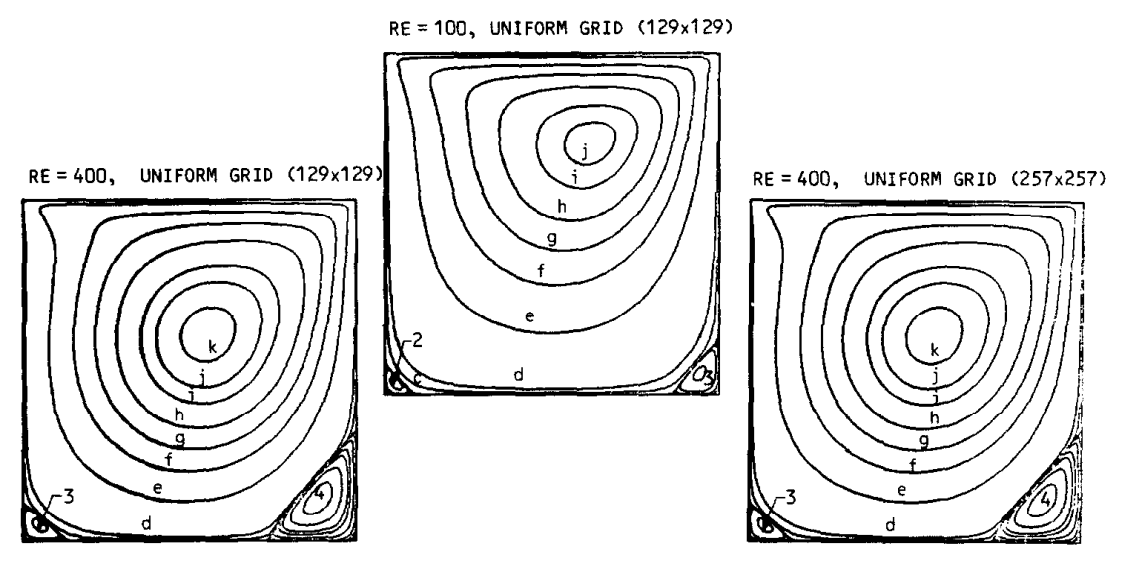
\includegraphics[width=.9\textwidth]{./img/ghia_solutions}
    \caption{Ghia's solutions for the lid-driven cavity flow at different Reynolds numbers.}
    \label{fig:ghia_solutions}
\end{figure}

\begin{figure}[H]
    \centering
    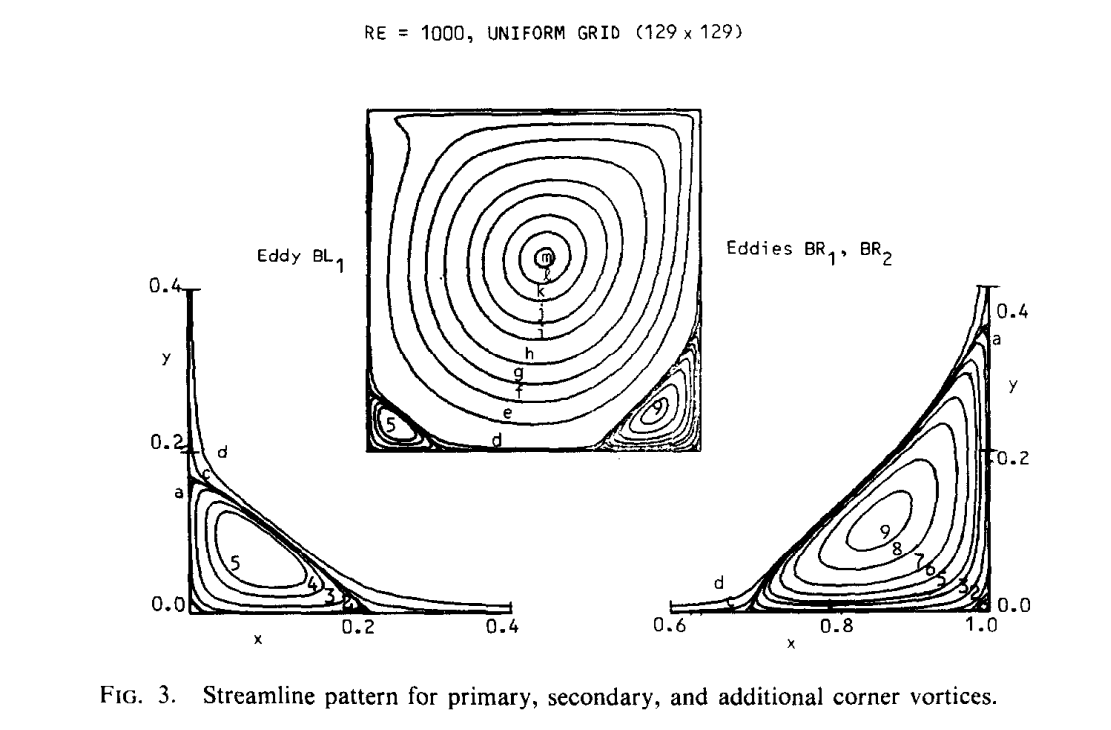
\includegraphics[width=.9\textwidth]{./img/ghia_solution_Re1000}
    \caption{Highlights of the eddy structures at the bottom corners of the cavity at $Re = 1000$.}
    \label{fig:ghia_solution_Re1000}
\end{figure}

We can now proceed with the comparison between our results and Ghia's solution.
\subsection{Comparison with Ghia's solution}
\label{subsec:comparison_with_ghia_solution}

Instead of just comparing the results by looking at the streamlines of the vector field which can be misleading, we are going to compare the velocity field at different points of the domain.
In particular, in Ghia's paper \cite{Ghia1982HighReSF} are reported the velocity profiles of $u(y) @ x/L_x = 0.5$ and $v(x) @ y/L_y = 0.5$ for different Reynolds numbers.

By using \texttt{MATLAB}, we can easily plot those profiles and compare them with the ones obtained using our code.

\textbf{Note:} to distinguish the different solutions generated by our code, we are going to use the following naming convention:

\begin{equation}
    \text{\#\#-Nx-Ny-Re-ConvectionScheme-DiffusionScheme-}\alpha_u\text{-}\alpha_v
\end{equation}

Where:

\begin{itemize}
    \item \#\# is the ID of the solution;
    \item $Nx$ is the number of points in the $x$ direction;
    \item $Ny$ is the number of points in the $y$ direction;
    \item $Re$ is the Reynolds number;
    \item $ConvectionScheme$ is the convection scheme used;
    \item $DiffusionScheme$ is the diffusion scheme used;
    \item $\alpha_u$ is the under-relaxation factor for the $u$ velocity (e.g. 08 for 0.8, 005 for 0.05, etc.);
    \item $\alpha_v$ is the under-relaxation factor for the $v$ velocity (e.g. 08 for 0.8, 005 for 0.05, etc.).
\end{itemize}

By benchmarking our code with different parameters, we have obtained the following velocity profiles.

\def\names{{00-40-40-100-UDS-SECOND-08-08},%
    {01-40-40-400-UDS-SECOND-008-008},%
    {02-40-40-1000-UDS-SECOND-008-008},%
    {04-40-40-1000-QUICK-SECOND-008-008},%
    {05-80-80-1000-UDS-SECOND-008-008},%
    {07-80-80-1000-QUICK-SECOND-008-008},%
    {08-129-129-1000-UDS-SECOND-008-008},%
    {09-129-129-1000-CDS-SECOND-008-008},%
    {10-129-129-1000-QUICK-SECOND-008-008},%
    {11-129-129-1000-UDS-FOURTH-008-008},%
    {12-129-129-1000-CDS-FOURTH-008-008},%
    {13-129-129-1000-QUICK-FOURTH-008-008}}

\foreach \name in \names {
    \begin{figure}[H]
        \includegraphics[width=\linewidth]{./img/ghia_comparison/\expandafter\name}
        \caption{Velocity comparison for solution \name.}
    \end{figure}
}

\subsection{07-80-80-1000-QUICK-SECOND-008-008}
\label{subsec:solution_07}

Considering just only the results obtained for $Re = 1000$, it is easy to see how \texttt{07-80-80-1000-QUICK-SECOND-008-008} is the one that better approximates the exact solution reported by Ghia et al. \cite{Ghia1982HighReSF}.

In the following figure we report all the data results obtained for the simulation runned with the following parameters:

\begin{table}[H]
    \centering
    \begin{tabular}{|c|c|}
        \hline
        \textbf{Variable} & \textbf{Value} \\ \hline
        Re                & 1000           \\
        Nx                & 80             \\
        Ny                & 80             \\
        $\alpha_u$        & 0.08           \\
        $\alpha_v$        & 0.08           \\
        Convection scheme & QUICK          \\
        Diffusion scheme  & SECOND         \\\hline
    \end{tabular}
    \caption{Parameters for simulation 07.}
    \label{tab:parameters_for_comparison}
\end{table}

\begin{figure}[H]
    \centering
    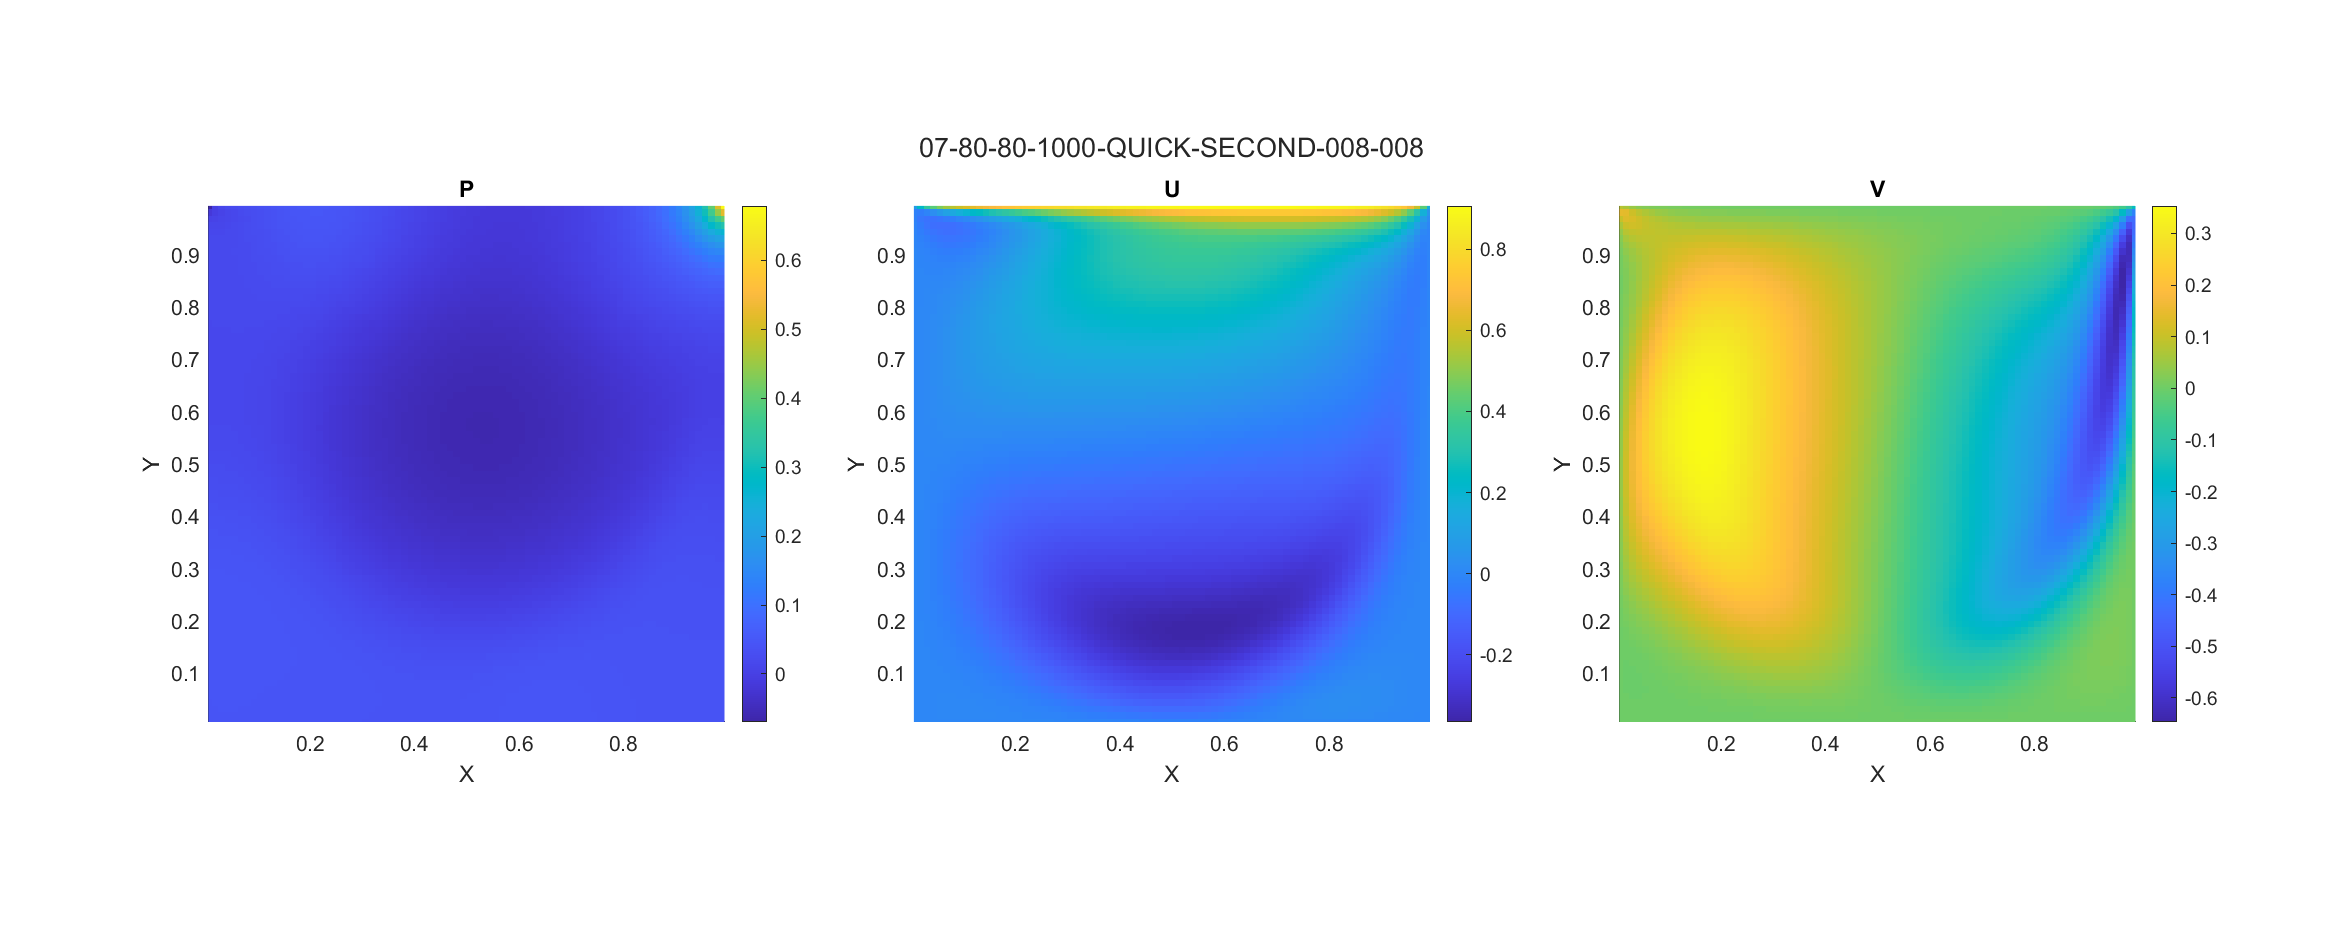
\includegraphics[width=\textwidth]{./img/states/07-80-80-1000-QUICK-SECOND-008-008}
    \caption{Final state of the simulation 07.}
    \label{fig:final_state_07}
\end{figure}

\begin{figure}[H]
    \centering
    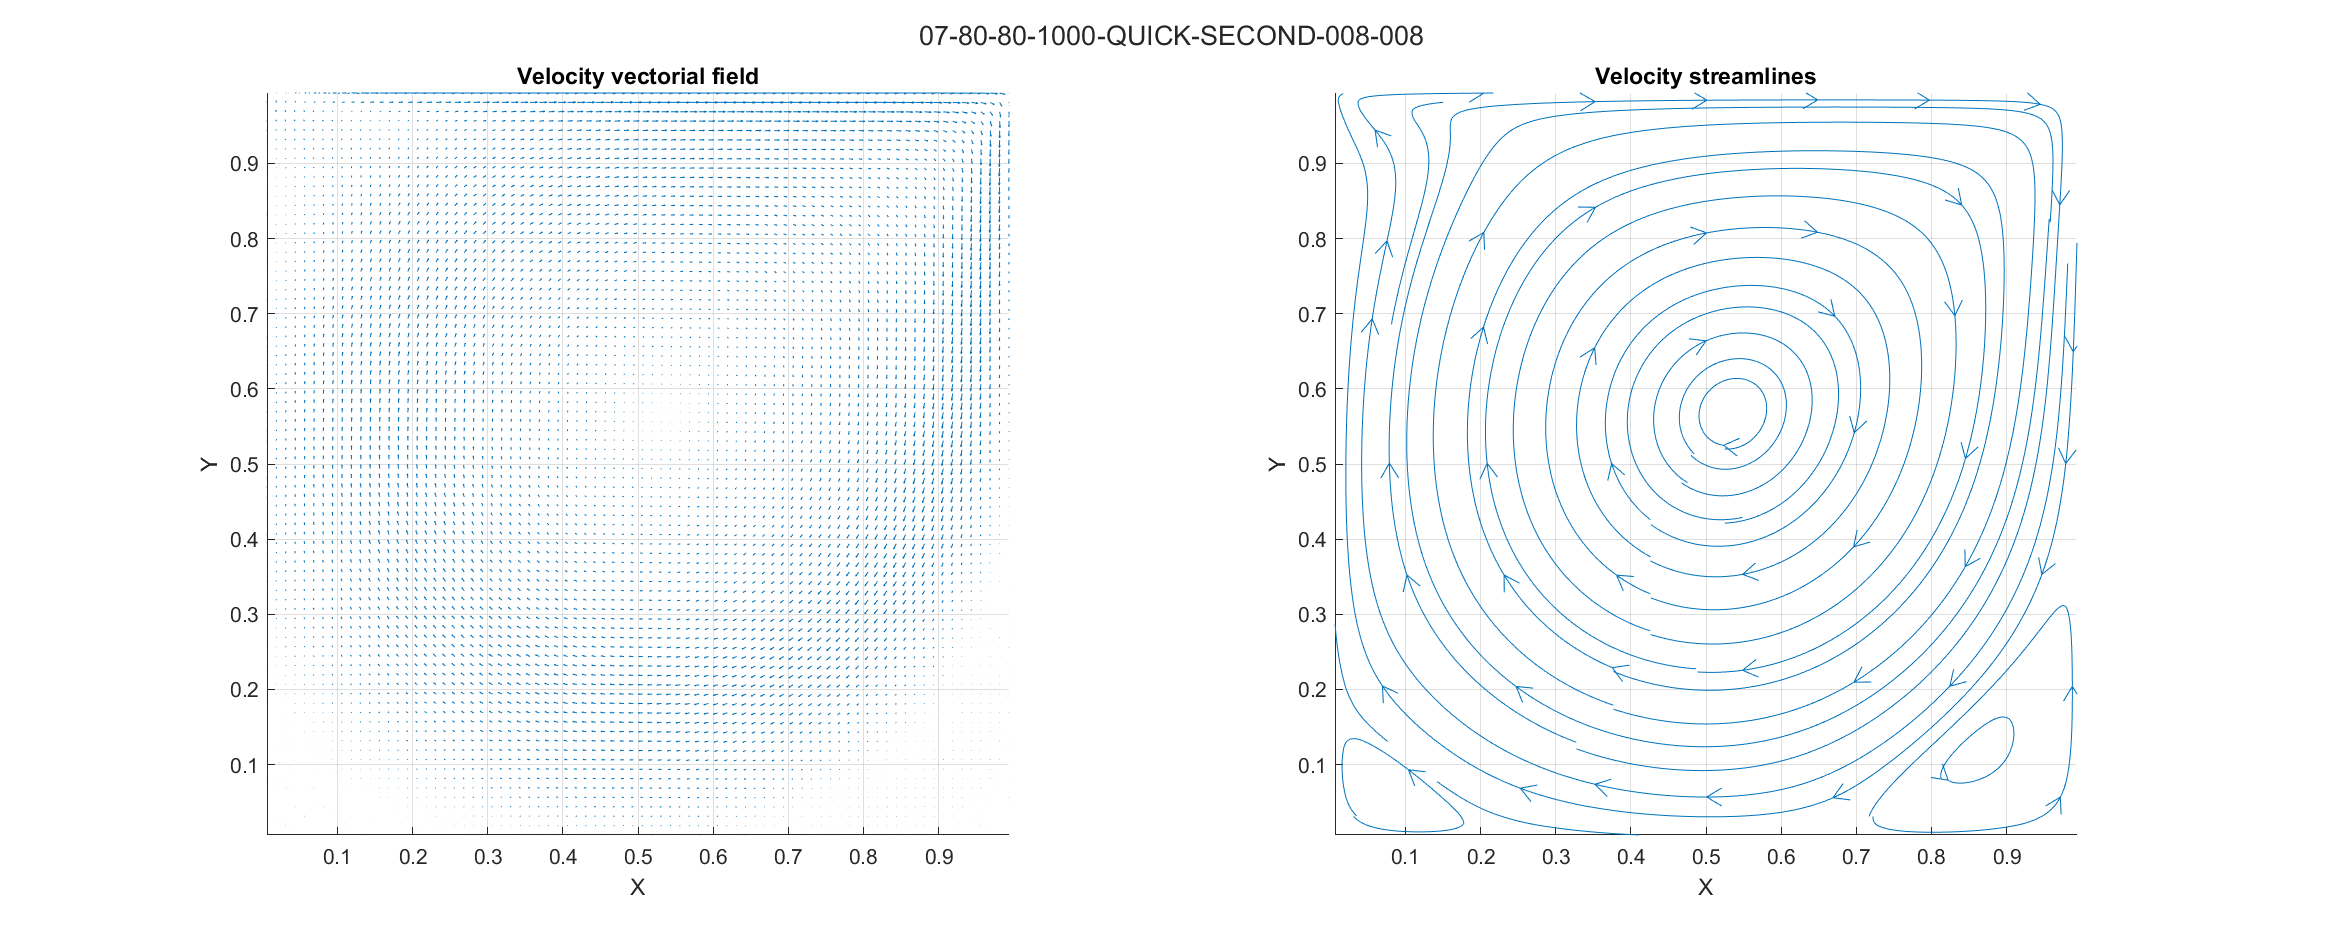
\includegraphics[width=\textwidth]{./img/streamline/07-80-80-1000-QUICK-SECOND-008-008}
    \caption{Streamlines of the simulation 07.}
    \label{fig:streamlines_07}
\end{figure}

\subsection{Convergence analysis}
\label{subsec:convergence_analysis}

In this section we report the convergence analysis of the \acrshort{scgs} algorithm.

\paragraph{Residual}

In Figure \ref{fig:residual} we report the residual of the algorithm for the different simulations runned.

\begin{figure}[H]
    \centering
    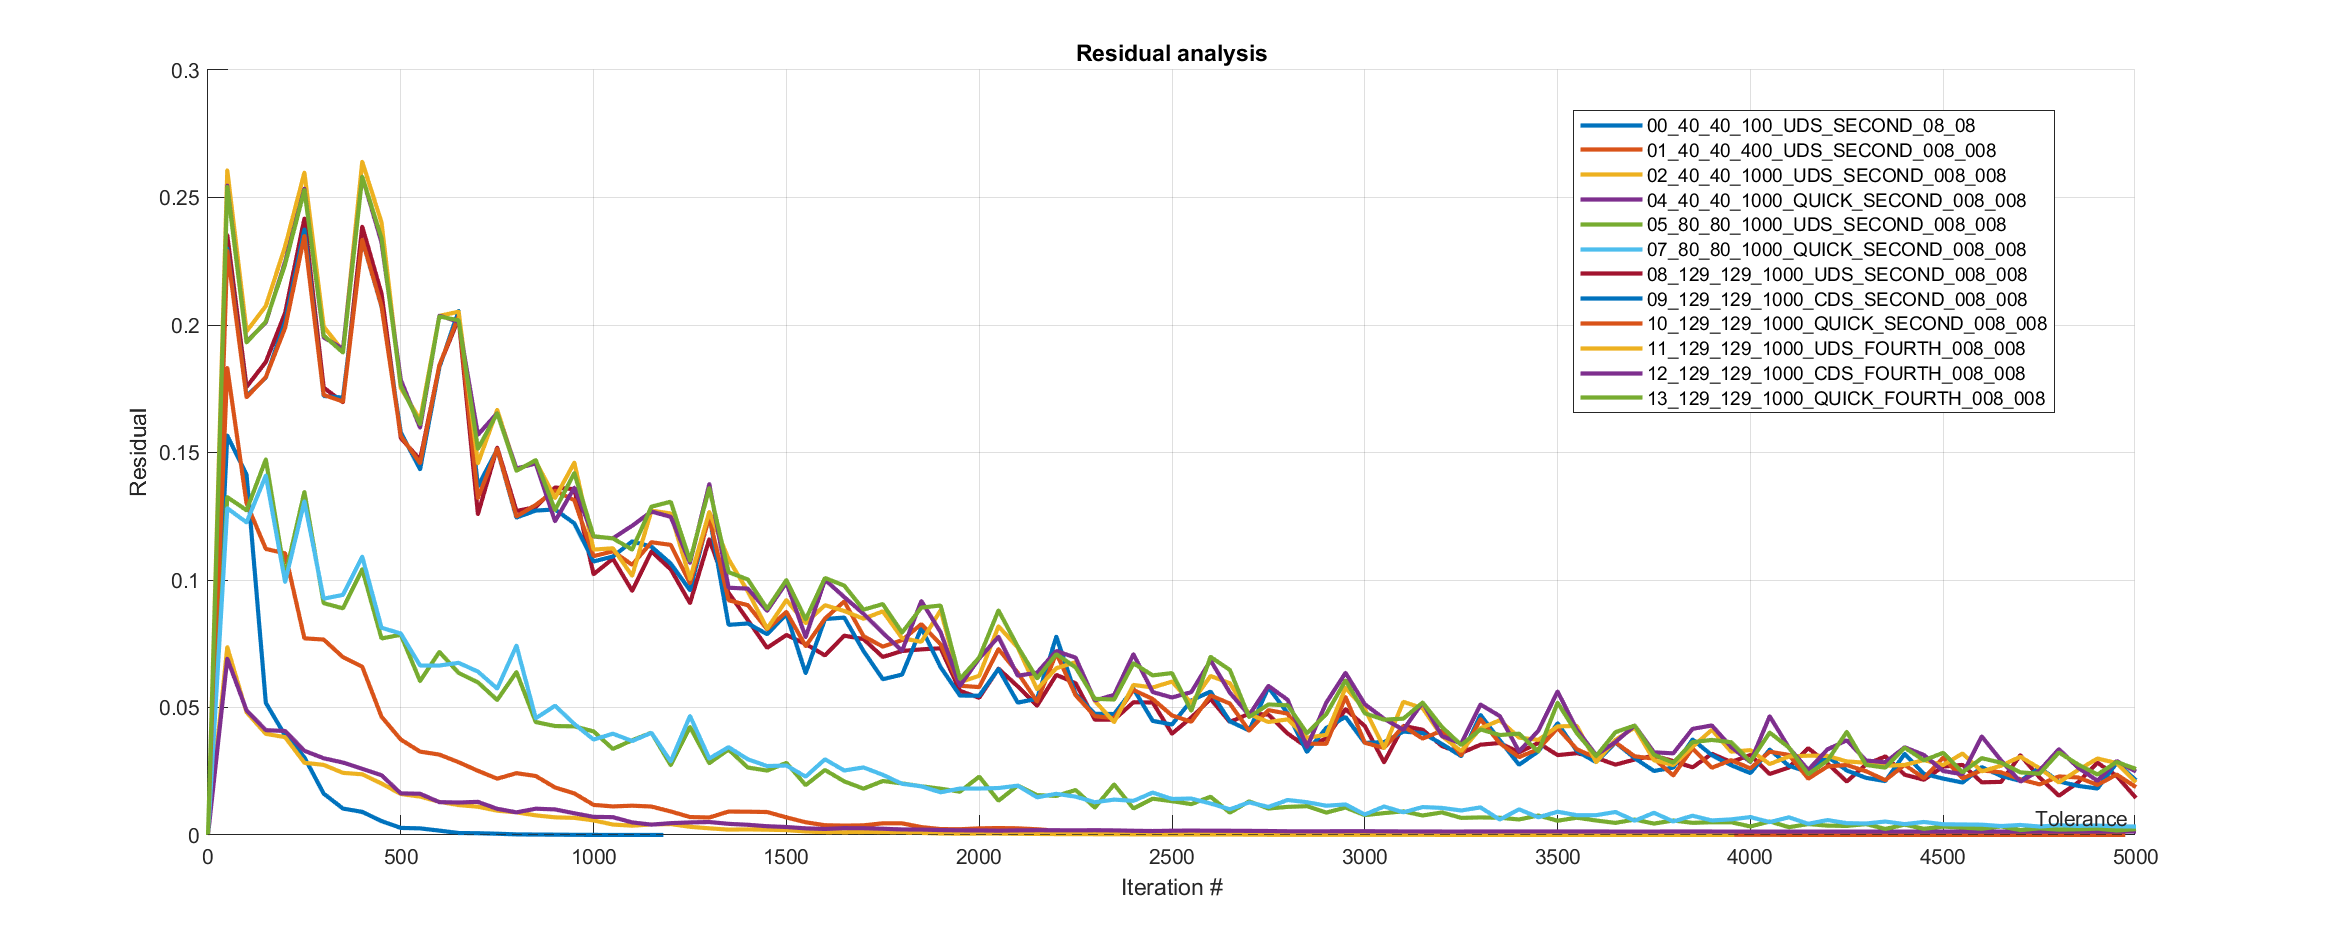
\includegraphics[width=\textwidth]{./img/residual}
    \caption{Residuals of the \acrshort{scgs} algorithm.}
    \label{fig:residual}
\end{figure}


\paragraph{CPU time}

In Figure \ref{fig:cpu_time} we report the CPU time of the algorithm for the different simulations runned.

\begin{figure}[H]
    \centering
    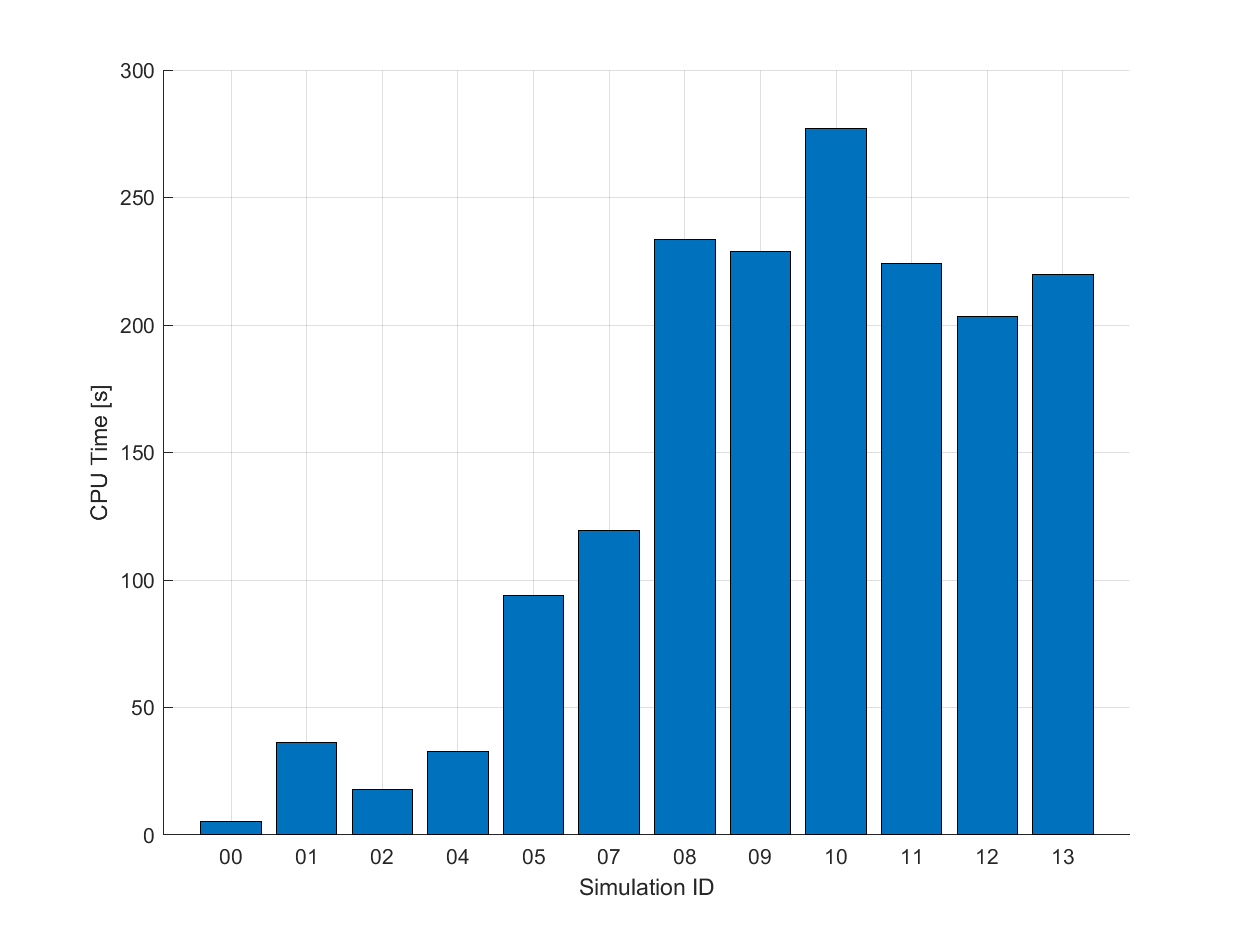
\includegraphics[width=\textwidth]{./img/CPU_time}
    \caption{CPU time of the \acrshort{scgs} algorithm.}
    \label{fig:cpu_time}
\end{figure}


\subsection{Final remarks}

As we have seen, our code has some issues related to convergence and stability.

In particular, in order to have a convergent solution, we have to decrease the under-relaxation factors to very low values (e.g. $\alpha_u = 0.01$ and $\alpha_v = 0.01$ or less).

By debugging through the code, we can clearly see that this is due to the low or absent diagonal dominance of the coefficient matrix (Vanka's matrix).

Moreover, by deepening the problem, we have found that the convergence of the algorithm is ensured only if the following condition is satisfied:

\begin{equation}
    |a_{ii}| \geq \sum_{j \neq i} |a_{ij}| \quad \forall i = 1, 2, 3, 4
    \label{eq:diagonal_dominance}
\end{equation}

Where $a_{ij}$ are the elements of the coefficient matrix.

In the \acrshort{scgs} algorithm the coefficient matrix is in the form of Equation \ref{eq:vanka_matrix}, so we can states that the diagonal dominance is ensured only if the following condition is satisfied:

\begin{equation}
    |a_{ii}| \geq |a_{5i}| \quad \forall i = 1, 2, 3, 4
\end{equation}

For how the system has been constructed, we know that:

\begin{align}
    a_{ii} & = f(\nu, \alpha_u, \alpha_v) \\
    a_{5i} & = f(Nx, Ny)
\end{align}

Where $f$ indicate a generic function.

Based on the equations and derivations done in the previous sections, we have that diagonal dominance is compromised when:

\begin{itemize}
    \item The grid is not fine enough (i.e. $Nx$ and $Ny$ are low) $\Rightarrow a_{5i} = \text{Cell sixe}$ is high
    \item The under-relaxation factors are high $\Rightarrow a_{ii} = A_p^\phi / \alpha_\phi$ is low
    \item The viscosity is low $\Rightarrow$ Diffusion term is low $\Rightarrow a_{ii}$ is low
\end{itemize}

When Equation \ref{eq:diagonal_dominance} is not satisfied once, then the algorithm will diverge imposing too high corrections to the state variables, causing the Convective terms to become too high at the next iteration (or neighboring cells).

\vspace{1em}

\textbf{Note: we know this should not append, but as of today we still haven't found the problem in our code.}

